% !TeX root = ../main.tex
% Add the above to each chapter to make compiling the PDF easier in some editors.

\chapter{Implementation}\label{chapter:implementation}

\section{Project Setup}

The projects as well as this thesis' source code are avaibable in the following Github repository:

\url{https://github.com/mulsicpp/bachelor_thesis_2025.git}

The project is organized in the following directories:

\begin{itemize}
    \item "assets": This folder contains the projects' assets. It is further divided into scenes, which contains the glTF test scenes, and "shaders", which contains the shaders, that are used in the different pipelines.
    \item "external": This folder contains all of the "complex""" external libraries. "Complex" in this context means, that the library has multiple header or source files or it is in binary form.
    \item "premake": This folder contains the premake executables for both windows and linux.
    \item "src": This folder contains all of our source files for the project. It is described in more detail in the next chapter.
\end{itemize}

Additionally, there are some scripts, that are used to build the project.

\subsection{Source Code Organization}

In this section we will specifically look at how the "src" folder is organised.

Directly in the "src" folder we find "main.cpp", which contains our entry point of the application.
The "external" folder once again contains external libraries, but this time the libraries, which are in the form of a single header file. These usually need to be included in a C/C++ file and need to be compiled. That's why it makes sense to keep these libraries with our other source files.
The "utils" folder contains utilities, that may be useful all throughout the project. It includes functionalities like debug logging, move semantics and file loading.
All the folders with a "vk\_" prefix contain code, which abstracts the low-level Vulkan API code. The goal of these abstractions is, that the low-level code should only ever be used in these folders. The rest of the project should only use the abstracted API. Each of the folders focuses on a different area of Vulkan:

\begin{itemize}
    \item "vk\_core": The most important class in this folder is the \texttt{Context} class. It is designed as a singleton, which contains the \texttt{VkInstance}, \texttt{VkPhysicalDevice}, \texttt{VkDevice}, \texttt{VkQueues} and \texttt{VmaAllocator}. After the context gets created it can be accessed anywhere. The folder also contains the \texttt{Handle<T>} class, which ensures that a handle only has one owner, the \texttt{CommandBuffer} abstraction and functionality to deals with \texttt{VkFormat}.
    \item "vk\_resources": This folder contains Vulkans resource objects like \texttt{Buffer} and \texttt{Image}, as well as \texttt{ImageView} and \texttt{SubBuffer}.
    \item "vk\_pipeline": This folder contains Vulkan objects, that are related to the setup of a pipeline. This includes \texttt{Pipeline}, \texttt{PipelineLayout}, \texttt{Shader}, \texttt{RenderPass}, \texttt{Framebuffer} and \texttt{DescriptorPool}.
    \item "vk\_sync": Contains the vulkan synchronization objects \texttt{Fence} and \texttt{Semaphore}.
    \item "scene": This folder contains the \texttt{Scene} class, which describes a dynamic scene with a scene graph. All the other classes used by or contained in the scene, like \texttt{Mesh}, \texttt{Node}, \texttt{Camera} and \texttt{Animation}, can also be found in this folder.
    \item "rendering": This folder contains 3 different renderers:
    \begin{itemize}
        \item \texttt{Rasterizer}: Render a scene from the viewpoint of a camera into a framebuffer using traditional rasterisation.
        \item \texttt{Raytracer}: Render a scene from the viewpoint of a camera into an image using modern hardware-accelerated raytracing.
        \item \texttt{Skinner}: Calculates the skinned positions of a mesh during an animation.
    \end{itemize}
\end{itemize}


\section{Move Semantics}
As already mentioned in the Methods and Technology chapter, Rust was originally considered as programming language, because it is modern and memory safe. One of Rust's core features is ownership, which means that each value/object can only be owned and managed by only one variable, and when that variable goes out of scope, it alone is responsible for cleaning up the object. When that variable gets assigned to another variable, the new variable becomes the new owner (i.e. the value gets moved). Ownership would be a very nice feature to manage \getVkObjects{}. \getVkObjects{} should not be copied on assignment but only moved and when the object is no longer needed (i.e. the owner goes out of scope), it should automatically be destroyed.
While C++ does not support ownership directly, it does have so-called move semantics, with which we can emulate ownership. The ownership of Vulkan handles is managed by the \texttt{Handle<T>} class. To do this the class declares a default constructor, move constructor and destructor and overrides the move assignment operator. It is also important, that the copy constructor and copy assignment operator are deleted. The reason for that is that copying a \getVkObject{} is usually very expensive or not even possible and it is almost never necessary. When we want to copy an object, we need to explicitly create a new one first. This avoids unnecessary and complicated accidental creation and copying of new objects.

\section{Shared Pointers}
Since C++11 the language supports so-called smart pointers, which make memory management safer and less complicated. One of these smart pointers is \texttt{std::shared\_ptr<T>} (or our alias \texttt{ptr::Shared<T>}). This type of pointer allocates an object, which can then be shared between multiple owners. The object lives while it has at least one owner, and the last object to go out of scope cleans up the object. This structure can be combined very nicely with our previously defined handle. A \getVkObject{} can only have one owner, which is a harsh limitation and often causes problems. If we wrap the object in a shared pointer, it can be shared across multiple owners. We also added the class \texttt{ToShared<T>}, which a class can inherit from. An instance of that class can then be moved into a shared pointer by calling \texttt{to\_shared()}.

\section{The Builder Pattern}
As mentioned, before we want the creation of \getVkObjects{} to be very explicit. The first method to create objects in C++ you think of are constructors, but they prove to be problematic for a couple of reasons. The first problem is that constructors are often called implicitly (e.g. the default constructor gets called when declaring a variable). Default construction only makes sense for very few \getVkObjects{} (like for example a VkFence) and we do not want a \getVkObject{} to be created when implicitly (or explicitly) calling the default constructor. So, for that reason, the default constructor simply does not create a \getVkObject{} or, in other words, leaves the handle at \texttt{VK\_NULL\_HANDLE}. Now if a different constructor actually creates an object, the behavior of constructors becomes inconsistent regarding \getVkObject{} creation. In addition to that, \getVkObjects{} are almost always created using a \texttt{*CreateInfo} struct, which may take a lot of parameters. To solve all of these issues we implemented a \texttt{Builder} class for most \getVkObjects{}. Some exceptions are \texttt{Fence} and \texttt{ImageView}, which are created with \texttt{Fence::create(...)} and \texttt{ImageView::create\_from(...)} respectively. This makes it very clear when a \getVkObject{} is created, since it can only be created using a \texttt{Builder} or a static method (like \texttt{Fence::create(...)}) and especially it can never be created by a constructor. This is also the reason \getVkObjects{} never have constructor, besides the default constructor.

\begin{lstlisting}[language=C++]

vk::Buffer buffer; // declare a buffer (handle is VK_NULL_HANDLE)

buffer = vk::BufferBuilder()
    .add_usage(VK_BUFFER_USAGE_TRANSFER_DST_BIT)
    .add_usage(VK_BUFFER_USAGE_VERTEX_BUFFER_BIT)
    .memory_usage(VMA_MEMORY_USAGE_GPU_ONLY)
    .size(128)
    .build();


\end{lstlisting}

\section{The Vulkan Context}

Before we can actually do any work in Vulkan, we need to do a lot of setup. This usually includes the following steps:

\begin{enumerate}
    \item Create a \texttt{VkInstance}.
    \item Select a \texttt{VkPhysicalDevice}, which supports the extenstions, features and capabilities required by the project.
    \item Create a \texttt{VkDevice} from the selected \texttt{VkPhysicalDevice}.
    \item When creating the \texttt{VkDevice}, \texttt{VkQueue}s from a certain queue family need to be enabled, to be able to submit command buffers later.
\end{enumerate}

These \getVkObjects{} are accessed very frequently throughout the project. For example, you need to pass the \texttt{VkDevice} as a parameter when creating or destroying most \getVkObjects{} and a command buffer, which executes a sequence of Vulkan commands, needs to be submitted to a certain \texttt{VkQueue}. Keeping track of all of these \getVkObjects is quite tideous, which is why we introduced the Vulkan context. It is represented by the \texttt{vk::Context} class, which stores these \getVkObjects, allows the programmer to access them anywhere and reduces the effort of stting up Vulkan.

The Vulkan context contains the following objects:

\begin{itemize}
    \item the \texttt{VkInstance}
    \item the \texttt{VkPhysicalDevice} and \texttt{VkDevice}
    \item an optional \texttt{GLFWwindow*} from which a \texttt{VkSurfaceKHR} is created and also stored (this is necessary for rendering to a window, but it will not be used in our main application, since it is headless)
    \item the \texttt{vk::CommandManager}
    \item the \texttt{VmaAllocator}
\end{itemize}

The class is designed similar to a singleton, but it deviates in some parts. A singleton usually creates its instance at the start of the application or when it is used for the first time (lazy instantiation). However, \texttt{vk::Context} can not be implicitly instanciated this way, because it needs some parameters stored in a \texttt{vk::ContextInfo}, when being instanciated. For this reason we need to explicitly create the Vulkan context using \texttt{vk::Context::create(...)} with the desired \texttt{vk::ContextInfo} before calling \texttt{vk::Context::instance()} for the first time or we will get a \texttt{nullptr}. While all other objects in our project get cleaned up automatically when going out of scope, the Vulkan context also needs to be destroyed explicitly using \texttt{vk::Context::destroy()} when it is no longer needed. If we now want to get the current \texttt{VkDevice}, we can call \texttt{vk::Context::instance()->get\_device()}.

\section{The Command Manager}

Queue management in Vulkan is a big and complex topic. Vulkan exposes the different queue families on your GPU, which support a subset of the following command types:

\begin{itemize}
    \item Graphics
    \item Transfer
    \item Compute
    \item Present
\end{itemize}

When submitting a command buffer to a queue, the queue needs to belong to a queue family, which supports the different types of the commands in the command buffer.

The management of Vulkan queues is completly up to the programmer. You can query the capabilities of the queue families and then enable an arbitrary amount of queues from different queue families. This is especially useful in a multi-threaded application, where you can submit two command buffers to two different queues and they will be executed in parallel.

The \texttt{vk::CommandManager} class makes queue management easier. It manages the queue families, aswell as their enabled queues and created descriptor pools. Our application is signle-threaded in order to avoid too much complexity and because our main objective is to benchmark the performace of dynamic raytracing, which works better in a single-threaded environment. For this reason we also do not need multiple queues or queues designated for a certain type of operations (for example a designated transfer queue). However we do need a queue for every command type, which our command manager ensures. For every command type, it will iterate over all queue families and select the first family, which supports the command type. When creating the device, we enable the first queue of every queue family, which has been selected at least one time for a command type.

The following are some examples of possible queue setups:

\begin{figure}[H]
    \centering
    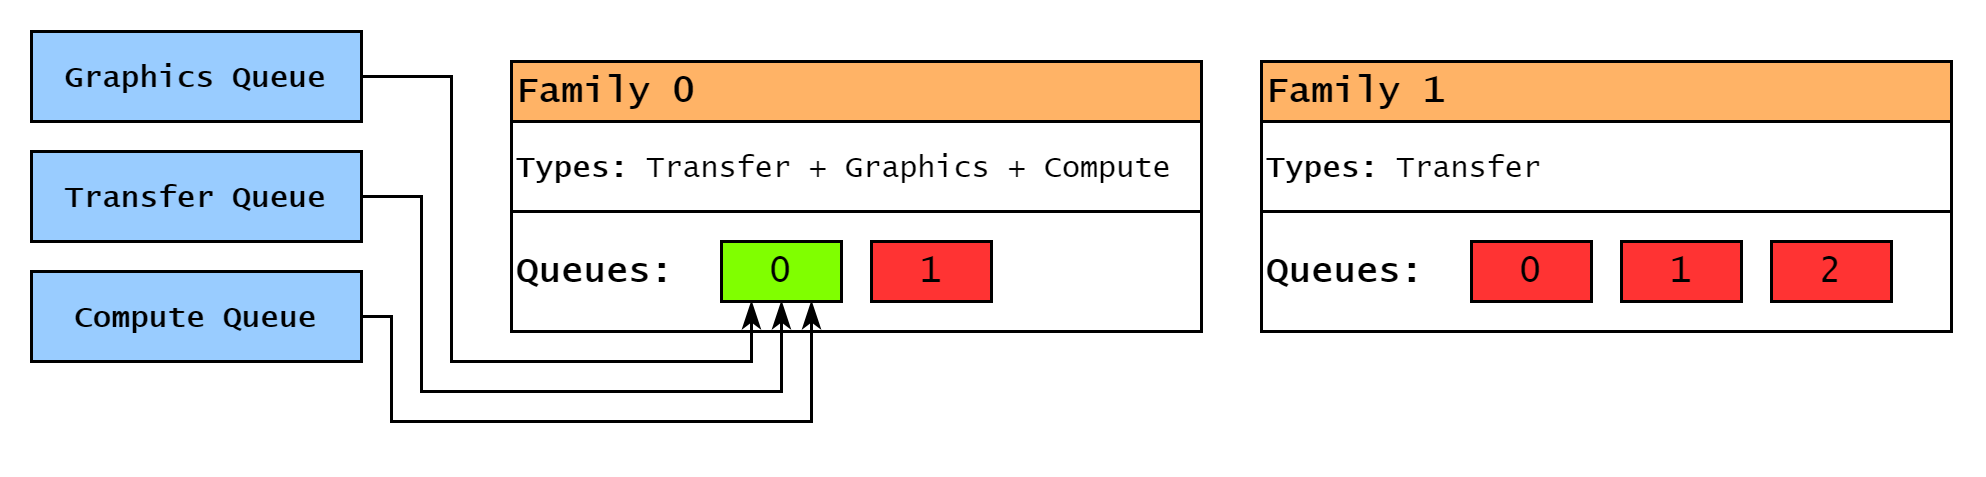
\includegraphics[width=1.0\textwidth]{figures/queue_setup_example_1.png}
    \caption{Queue setup example with only one queue}
    \label{fig:queue-example-1}
\end{figure}

\begin{figure}[H]
    \centering
    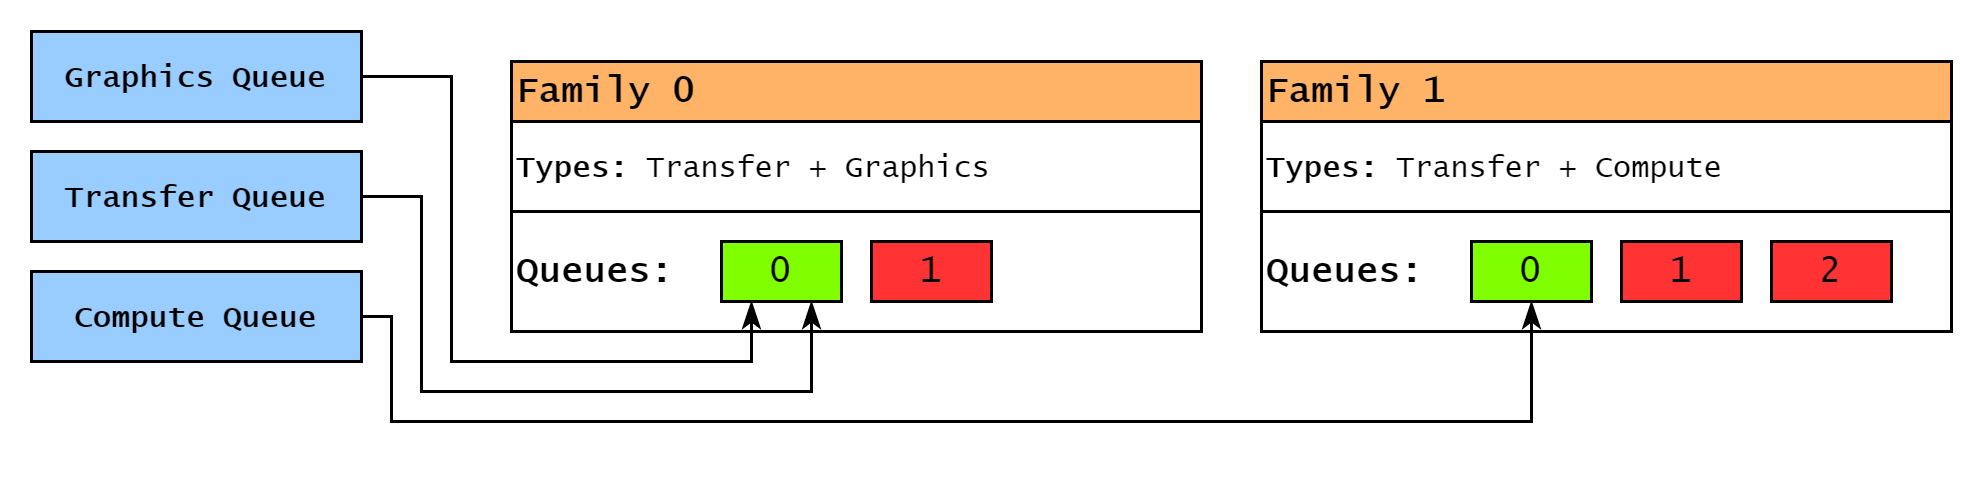
\includegraphics[width=1.0\textwidth]{figures/queue_setup_example_2.png}
    \caption{Queue setup example with two queues}
    \label{fig:queue-example-2}
\end{figure}

We also need a command pool to be able to allocate command buffers. When creating a command pool, a queue family has to be specified. Because the allocated command buffers can only be submitted to queues of the specified family, we create one command pool for every queue family that is used.

\section{The VMA Allocator}

As already mentioned in the chapter \nameref{chapter:technologies} (\autoref{sec:vma}), our project uses VMA (Vulkan Memory Allocator) to make memory management in Vulkan easier. In order to be able to be allocate memory for our buffers and images later, we need an allocator. The allocator should be easily accessible when we create a buffer or image and for that reason we will also create and store the VMA allocator in the Vulkan context. We will use this allocator later, when allocation our resource objects (see \autoref{sec:resource_objects}).

\section{Command Buffers}

As we know, commands can not be executed in Vulkan directly, like they can for example in OpenGL. Instead, you first need to allocate a command buffer from a command pool. You can then record all of the commands you want to execute into the buffer and can then submit it for execution to a queue, that supports the type of the commands. It is important to note that when you submit the command buffer the current CPU-thread does not wait for all the commands to finish. This allows for the CPU to keep working, while the GPU runs our commands. If we want to wait for the command buffer to finish, we can specify a fence when submitting the command buffer, which will be signaled once all commands have finished.

We abstract this logic in the \texttt{vk::CommandBuffer} class. It contains a \texttt{VkCommandBuffer} handle, a \texttt{vk::Queue}, which tells the command buffer, where it should be submitted to, and a \texttt{vk::Fence} (see \autoref{sec:sync_objects}), which is used to wait for the command buffer to finish executing.

The \texttt{vk::CommandBufferBuilder} has the following two parameters:

\begin{itemize}
    \item \textbf{\texttt{queue\_type}}: A value of type \texttt{vk::QueueType}, which contains the elements \texttt{Transfer}, \texttt{Graphics}, \texttt{Compute} and \texttt{Present}. It is a mandatory parameter, which tells the builder to which of the queues inside the queue manager the command buffer is going to be submitted to (for example \texttt{vk::QueueType::Graphics} means the command buffer will be submitted to the graphics queue of the command manager).
    \item \textbf{\texttt{single\_use}}: An optional boolean value, which is set to \texttt{false} by default. If set to \texttt{true}, it sets the \texttt{VK\_COMMAND\_BUFFER\_USAGE\_ONE\_TIME\_SUBMIT\_BIT} flag when recording the command buffer. This flag specifies, that the command buffer will only be submitted once, which lets the driver apply optimizations.
\end{itemize}

Inside \texttt{vk::CommandBuffer} we can find the following member functions:

\begin{itemize}
    \item \textbf{\texttt{Ref record(vk::CommandRecorder)}}:
    
    This function takes in a \texttt{vk::CommandRecorder} as argument, which is an alias for \break \texttt{std::function<void(vk::ReadyCommandBuffer)>}. In other words it is a function pointer or lambda function, which takes a \texttt{vk::ReadyCommandBuffer} as an argument and returns \texttt{void}. A \texttt{vk::ReadyCommandBuffer} is simply a wrapper around a \texttt{VkCommandBuffer} handle, which can only be constructed by the command buffer. The job of the \texttt{vk::CommandRecorder} is, to record commands into the command buffer.

    Functions, that record a commands can be recognized by their \texttt{"cmd\_"} prefix. These functions have to be called inside a \texttt{vk::CommandRecorder}, because thier first argument is always a \texttt{vk::ReadyCommandBuffer}.

    \item \textbf{\texttt{Ref submit(vk::SubmitInfo)}}:
    
    This function submits the command buffer to the queue, for which it was created for. The \texttt{vk::SubmitInfo} parameter is optional and empty by default. This parameter allows us to specify semaphores, that we want to wait for before executing the command buffer, and semaphores, that we want to signal once the command buffer is finished executing (see \autoref{sec:sync_objects}).

    \item \textbf{\texttt{Ref wait()}}:
    
    This functions simply waits for the execution of the command buffer to finish using a fence. If the command buffer is not currently getting executed, the function does nothing.

    It is also important to mention, that this function also gets called in the desctructor of the \texttt{vk::CommandBuffer}, since it is not allowed to destroy a \texttt{VkCommandBuffer} while it is in execution. This also means, that a command buffer implicitly wait for execution to finish, when it goes out of scope.
\end{itemize}

The \texttt{vk::CommandBuffer} class also contains the following static method:

\begin{center}
    \textbf{\texttt{static void single\_time\_submit(vk::QueueType, vk::CommandRecorder)}}
\end{center}

It creates a single-use command buffer for the queue with the specified \texttt{vk::QueueType}. Then, it records the given \texttt{vk::CommandRecorder}, submits it with an empty \texttt{vk::SubmitInfo} and waits for execution to finish. It is basically just a quality-of-life function for creating and executing single-use command buffers.

The folloing code snippet shows, how the command buffer and its functions can be used:

\begin{figure}[H]
\centering
\begin{tabular}{c}
\begin{lstlisting}[language=C++]

// create the command buffer
vk::CommandBuffer cmd_buf = vk::CommandBufferBuilder()
    .queue_type(vk::QueueType::Graphics)
    .single_use(true)
    .build();

// create a callback, which records the commands
vk::CommandRecorder recorder = [&] (vk::ReadyCommandBuffer ready_buf) {
    // record commands
    // ...
}

// record the commands, submit to queue and 
// wait for execution to finish in one line
cmd_buf.record(recorder).submit().wait();


\end{lstlisting}

\end{tabular}
\caption{An example of how to use command buffers in your code.}\label{fig:command-buffer}
\end{figure}

\section{Resource Objects}\label{sec:resource_objects}
\textbf{Resource objects} are used to store data on the GPU, which can then be read and written to in shaders. In Vulkan we distinguish two types of resource objects:

\begin{itemize}
    \item \textbf{Buffer:}
    
    Buffers represent linear arrays of data which are used for various purposes by binding them to a graphics or compute pipeline via descriptor sets or certain commands, or by directly specifying them as parameters to certain commands~\parencite[see Section~12.1]{vulkan-spec}. The data is raw and not associated with any format, layout or dimensionality, therefore very flexible.

    Common usages:
    \begin{itemize}
        \item Vertex buffer
        \item Index buffer
        \item Uniform buffer
        \item Storage buffer
    \end{itemize}

    \item \textbf{Image:}

    Images are specialized resources that have multi-dimensional access rather than the typical linear access to memory~\parencite[see Section~13]{vulkan-spec}. They can also be multi-dimensional and are associated with a format and layout.
    
    Common usages:
    \begin{itemize}
        \item Texture
        \item Render target
    \end{itemize}
\end{itemize}

We represent these two objects by the \texttt{vk::Buffer} class and {vk::Image} class. Since they are both resource objects, they are very similar in certain aspects. One challange, that they both share, is memory management, which can be quite difficult.

When creating a resource object, they are not actually backed by memory immediately, but you need to allocate a block of device memory and bind that memory to the resource. When allocating the memory, you need to specify a memory type, which corresponds to a certain memory heap and can have a set of properties, which impact the visibility of your memory aswell as performance. It is also important to mention, that too many allocations are not just bad for the performance of your application, but there is also a limit of allocations, that cannot be superceeded.

To make our lives a little bit easier, we use VMA (Vulkan Memory Allocator) (see \autoref{sec:vma}). 

\section{Synchronization Objects}\label{sec:sync_objects}

A lot of vulkan operations can be executed in parallel, which is why we need synchronization objects. There are two types:

\begin{itemize}
    \item \textbf{Semaphore:}
    
    A semaphore is used to synchronize two operations, which both happen on the GPU. We do this by specifying and array of wait-semaphores and an array of signal-semaphores. The GPU operation waits for all wait-semaphores to be signaled before starting and signals all signal-semaphores when it is finished.

    \item \textbf{Fence:}
    
    A fence is used to synchronize operations on the GPU with the CPU. This is done by specifying a fence when starting a GPU operation. When the GPU operation finishes, the fence gets signaled. The CPU can wait on a fence, which will block the thread until the fence gets signaled.
\end{itemize}